\section{Protocol Semantics}

% TODO: Distinguish operations from messages, make sure messages aren't signed.
% TODO: Make sure all operations, ex. around issues are using a message token.

The rules according to which transactions on the \oscoin{} network are
validated comprise a \emph{protocol}. This protocol has a well defined semantics
which we shall describe in this section.

\subsection{Overview} The \oscoin{} protocol is composed of interrelated
\emph{objects} which form a hierarchical graph as seen in Figure
\ref{object-relationships}, and \emph{operations}, which act on these objects.

\medskip

\begin{figure}[htp]
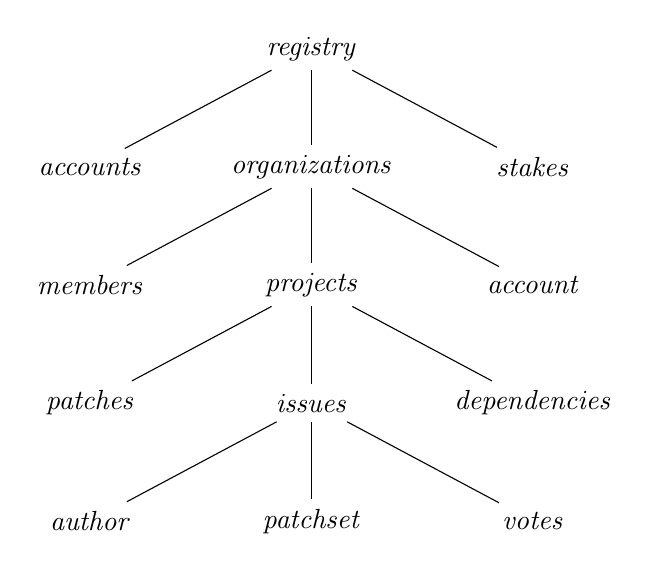
\begin{tikzpicture}[sibling distance=8em]
    \node {\emph{registry}}
        child { node {\emph{accounts}} }
        child { node {\emph{organizations}}
            child { node {\emph{members}} }
            child { node {\emph{projects}}
                child { node {\emph{patches}} }
                child { node {\emph{issues}}
                    child { node {\emph{author}} }
                    child { node {\emph{patchset}} }
                    child { node {\emph{votes}} } }
                child { node {\emph{dependencies}} } }
            child { node {\emph{account}} } }
        child { node {\emph{stakes}} };
\end{tikzpicture}
\bigskip
\caption{Object relationships in the \oscoin{} protocol.
\label{object-relationships}}
\end{figure}

\subsection{Operations}

Operations are signed messages constructed by participants in the protocol,
which trigger a state transition in the network. A valid operation $T$ takes
the form:
\[
    T \equiv \tuple{T_i, T_m, T_p, T_n}_{\sigma}
\]
where $T_i$ is the identity of the sender of the operation, $T_m$ is the
message, $T_p$ is a reference to a parent operation which $T$, such that $T_p
\prec T$, and $T_n \in \mathbb{N}$ taken together with $T_i$ forms a globally
unique operation identifier, such that there can be at most one operation with
a given $\tuple{T_i, T_n}$ tuple. In the remainder of the paper, we shall
use the word \emph{operation} to mean either a tuple $T$, or its message $T_m$.

A valid operation $T$ applied to the current state of
the protocol $\mathcal{S}_e$ at epoch $e$ can be formulated as:
\[
    \mathcal{S}_{e+1} \equiv \delta(\mathcal{S}_e, T)
\]
where $\delta$ is \emph{apply}, the state-transition function.  We can describe
the current state of the network $\mathcal{S}_e$ as a sequence of operations
$\mathcal{L} = T_1 \dots T_e$ applied recursively to an initial empty state
$\varnothing$:
\[
    \mathcal{S}_e \equiv \delta(\dots \delta(\delta(\delta(\varnothing,
    T_1), T_2), T_3), \dots T_e)
\]
The state $\mathcal{S}$ of the protocol is defined as:
\[
    \mathcal{S} \equiv \tuple{\mathcal{A}, \mathcal{O}, \mathcal{D}, \mathcal{L}} \\
\]
where $\mathcal{A}$ is the set of accounts (\ref{accounts}), $\mathcal{O}$ is
the set of organizations known to the protocol (\ref{orgs}), $\mathcal{D}$ is
the set of dependencies between projects (\ref{dependencies}) and $\mathcal{L}$
is the sequence of operations which have been applied to $\mathcal{S}$. It is
thus possible to reconstruct $\mathcal{S}$ from $\mathcal{L}$ via the $\delta$
function, as seen above.

\subsection{Patches}
\label{patches}

The fundamental product or \emph{artifact} of the \oscoin{} network is code, or
source code. Our protocol defines the \emph{patch} primitive as the atomic unit
of code. A patch is a set of metadata and code changes, or \emph{changeset},
that can be applied to an existing body of code, or \emph{context}, to modify
it. We define a patch $P$ as the tuple $\tuple{ P_a, P_m, P_f}$, where $P_a$ is
the author of the patch, $P_m$ is the patch metadata and $P_f$ is the
changeset. A set of patches in no particular order is called a \emph{patchset}.

Patches can be composed sequentially, taking an initial context $A$ into
a modified context $B$. The empty context is defined as $\varnothing$, such
that there exists a mapping $P_f \varnothing \mapsto P_f$. Let $f \prec g
\prec h$ be an ordered sequence of patches, then the formulation:
\[
h \cdot g \cdot f : A \to B
\]
is the in-order composition of patches $f$, $g$ and $h$, taking an initial
context from $A$ to $B$.

% TODO: Contexts form a free monoid?
% TODO: Reference patch theory.

\subsection{Issues}
\label{issues}

On the \oscoin{} network, collaboration on code takes place through \emph{issues};
and since project governance is specified in code---through the use of
\emph{smart contracts}---organizational decisions are also made through issues.

% TODO: Remove reference to smart contracts!

An issue $I$ is described at epoch $e$ by the tuple:
\[
    \big<\tuple{I_a, I_t, I_b, I_o, I_r, I_P}_{\sigma}, I_s, I_V \big>_e
\]
where $I_a$ is the issue author, $I_t$ is the title or subject of the issue,
$I_b$ is the description in plain text of the issue, $I_o$ is a list of
operations to be applied when $I_s$ changes, $I_r$ is the issue resolution
function, $I_P$ is the patchset attached to the issue, $\sigma$ is the
signature of $I_a$, $I_s \in \{open, closed, accepted, rejected\}$ is the
current state of the issue and $I_V$ is the set of votes on the issue. The
initial value of $I_s$, $I_{s_0} = open$, the initial value of $I_V$, $I_{V_0}
= \varnothing$ and the initial value of $I_P$, $I_{P_0} = \varnothing$.  A list
of valid state transitions between any two states $I_s$ and $I_{s'}$ can be
found in Table \ref{issues-valid-transitions}.

\begin{table}[hbt]
    \caption{Valid state transitions.\label{issues-valid-transitions}}
    \begin{tabular}{rcl}
        \toprule
        $I_s$      & $\to$ & $I_{s'}$ \\
        \midrule
        $open$     & $\to$ & $accepted$ \\
        $open$     & $\to$ & $rejected$ \\
        $open$     & $\to$ & $closed$ \\
        $closed$   & $\to$ & $open$ \\
        \bottomrule
    \end{tabular}
\end{table}

The patchset $I_P$ attached to an issue represents a set of proposed changes to
some project, while the subject $I_t$ and body $I_b$ of the issue provide a
description of the changes contained in $I_P$. Issue \emph{resolution} is the
process of voting on an issue with the aim to move to an \emph{accepted} or
\emph{rejected} state.

Issues can be voted on with the \textsc{voice} operation. When an issue receives
a new vote, it is added to $I_V$. A vote $v$ is represented by the tuple
$\tuple{v_i, v_a, v_{\omega}, v_e}_{\sigma}$ where $v_a$ is the voter,
$v_i$ is the issue being voted on, $v_{\omega} \in \{accept, reject\}$ and
$v_e$ is the epoch $e$ at which the vote is valid.

When a certain threshold of votes is reached, an issue transitions to either an
\emph{accepted} or \emph{rejected} state. Given an open issue $i$, the rules of
issue resolution are defined by the function $i_r : I \to I$, applied to the
issue $i$ for every vote added to $i_V$.

\subsubsection{Amendments}

An issue $I$ where $I_s = open$ can be amended with the \textsc{amend}
operation, or $\amend$. Only $I_t$, $I_b$, $I_o$, $I_r$ and $I_P$ can be
amended.  Amending an issue creates a new empty set of votes $V'$, ensuring two
versions of a given issue never share a set of votes. Formally, amendment is
defined as:
\begin{align*}
    I \amend{} \langle I_a, t', b', o', r', P' \rangle_{\sigma} \equiv
    \big<\langle I_a, t', b', o', r', P' \rangle_{\sigma}, I_s, \varnothing
    \big>, \qquad I_s = open
\end{align*}

% TODO: The amendment should include the issue it is amending.

\subsubsection{Accepted Issues} When an issue has been accepted by a majority
of votes, the issue transitions permanently into an \emph{accepted} state. The
steps taken by the protocol are as follows:

\begin{enumerate}
    \item The issue's state $I_s$ is set to \emph{accepted}.
    \item The issue is \emph{frozen}, such that no further amendments or state
        changes are possible.
    \item The list of operations $I_o$ belonging to the issue are executed by
        the protocol.
    \item The issue's \emph{patchset} $I_P$ is permanently added to the code
        project it pertains to. Note that a patchset may contain individual
        patches pertaining to different projects, in which case the patches are
        applied individually to their respective projects.
\end{enumerate}

\subsubsection{Rejected issues} When an issue is rejected,
\begin{enumerate}
    \item The issue transitions to a \emph{rejected} state.
    \item The issue is frozen so that no further amendments or state
        transitions are possible.
    \item The list of operations $I_o$ belonging to the issue are executed by
        the protocol.
\end{enumerate}

\subsubsection{Closed issues} When an issue is closed, its state changes to
\emph{closed} until it is re-opened. No operations from $I_o$ are run, since
an issue can be opened and closed many times. Only the author $I_a$ of an issue
can close it.

\subsection{Value}

To enable the transfer of value in the network, the protocol defines a scarce
currency we shall refer to in the remainder of this paper as~\coin{}, or
\oscoin{}.

\subsubsection{Supply}

The supply of \coin{} is subject to an inflation $e_{\iota} \in \mathbb{N}$,
carried out by the protocol every epoch $e$, and determined by a function $f :
e \to e_{\iota}$, such that
\[
    \lim_{e\to\infty} f(e) = 0
\]

\subsubsection{Accounts}
\label{accounts}

Currency is held in \emph{accounts} which can be unlocked by the signature of
the account holder. Accounts have addresses which are used to send and receive
\coin{}.

\subsubsection{Transfer}

Value can be transfered from one account to another with the \textsc{send}
message, formally defined as $\tx{send}{a_{s}, a_{r}, n}$, where $a_{s}$ and
$a_{r}$ are the \emph{sender} and \emph{recipient} address between which the
value should be transfered and $n$ is the value to transfer.  To be valid, a
\textsc{send} operation must be signed by the owner of $a_{s}$.

\subsubsection{Bonding}

Value can be locked in the system via an operation called \emph{bonding}.
This operation turns \emph{liquid} value into \emph{bonded} value, preventing
them from being moved for a certain amount of time, and can be used to perform
security deposits or other forms of commitment which require a collateral or
pledge. Bonding and unbonding operations are performed with the
\textsc{bond} and \textsc{unbond} messages defined as:
\[
    \tx{bond}{a, a_b, n} \qquad \tx{unbond}{a, a_b, n}
    \medskip
\]
where $a$ is the address from which to withdraw the value for bonding, $a_b$ is
the address where the value is to be bonded and $n$ is the value to bond. When
the \textsc{unbond} operation is used, an unbonding period $e_u$ is started,
measured in epochs. Once $e_{u}$ epochs have passed, the value is withdrawn
from the bonding address $a_b$ and credited back to $a$.

\subsection{Organizations}
\label{orgs}

An organization $O$ is described by the tuple:
\[
    \tuple{O_{id}, O_{a}, O_R, O_M}
\]
where $O_{id}$ is the organization's identifier, $O_a$ is its account, $O_R$ is
the set of repositories under $O$ and $O_M$ is the set of members belonging to
the organization. We can relate patches (\ref{patches}) and issues
(\ref{issues}) to repositories with the equations:
\begin{align*}
    O_R & \equiv \{R_1, R_2, \dots, R_n\}         \\
    R   & \equiv \tuple{R_{id}, R_I, R_P}         \\
    R_I & \equiv \{I_1, I_2, \dots, I_n\}         \\
    R_P & \equiv \tuple{P_1, P_2, \dots, P_n}
\end{align*}
where $R_{id}$ is the repository's identifier, $R_I$ is the set of issues
related to $R$, and $R_P$ is the sequence of patches composing its codebase.

The set $\mathcal{O} = \{O_1, O_2, \dots, O_n\}$ is the set of all organizations
known to the protocol.  Let $o$ be an organization, then $\tx{register}{o}$ is
an operation that registers $o$ and makes it known to the protocol such that:
\[
    \delta_o(\mathcal{O}, \tx{register}{o})
    \equiv \mathcal{O} \cup \{o\}
\]
where $\delta_o$ is a sub-function of $\delta$, and defines state-transitions
in $\mathcal{O}$.

\subsection{Dependencies}
\label{dependencies}

A project $a$ depends on a project $b$ at epoch $e$ if it could not function
without modification, were $b$ destroyed. Formally, we represent this as:
\[
    a \dep b
\]
Let $\accentset{*}{R}$ be the set $O_{1_R} \cup O_{2_R} \cup \cdots \cup
O_{n_R}$ of all projects accross all organizations, and $\mathcal{D}_e$ be the
set of all dependencies at epoch $e$, then:
\[
    \mathcal{D}_e \equiv \{(a, b) : a \in \accentset{*}{R}
    \land b \in \accentset{*}{R}
    \land a \dep b \}
\]
